\documentclass[12pt, titlepage]{article}

\usepackage{fullpage}
\usepackage[round]{natbib}
\usepackage{multirow}
\usepackage{booktabs}
\usepackage{tabularx}
\usepackage{graphicx}
\graphicspath{ {./UIMockups/} }
\usepackage{float}
\usepackage{hyperref}
\hypersetup{
    colorlinks,
    citecolor=blue,
    filecolor=black,
    linkcolor=red,
    urlcolor=blue
}

%% Comments

\usepackage{color}

\newif\ifcomments\commentstrue %displays comments
%\newif\ifcomments\commentsfalse %so that comments do not display

\ifcomments
\newcommand{\authornote}[3]{\textcolor{#1}{[#3 ---#2]}}
\newcommand{\todo}[1]{\textcolor{red}{[TODO: #1]}}
\else
\newcommand{\authornote}[3]{}
\newcommand{\todo}[1]{}
\fi

\newcommand{\wss}[1]{\authornote{blue}{SS}{#1}} 
\newcommand{\plt}[1]{\authornote{magenta}{TPLT}{#1}} %For explanation of the template
\newcommand{\an}[1]{\authornote{cyan}{Author}{#1}}

%% Common Parts

\newcommand{\progname}{Software Engineering} % PUT YOUR PROGRAM NAME HERE
\newcommand{\authname}{Team 2, SyntaxSentinals
\\ Lucas Chen
\\ Dennis Fong
\\ Mohammad Mohsin Khan
\\ Julian Cecchini
\\ Luigi Quattrociocchi} % AUTHOR NAMES                  

\usepackage{hyperref}
    \hypersetup{colorlinks=true, linkcolor=blue, citecolor=blue, filecolor=blue,
                urlcolor=blue, unicode=false}
    \urlstyle{same}
                                


\newcounter{acnum}
\newcommand{\actheacnum}{AC\theacnum}
\newcommand{\acref}[1]{AC\ref{#1}}

\newcounter{ucnum}
\newcommand{\uctheucnum}{UC\theucnum}
\newcommand{\uref}[1]{UC\ref{#1}}

\newcounter{mnum}
\newcommand{\mthemnum}{M\themnum}
\newcommand{\mref}[1]{M\ref{#1}}

\newcounter{smnum}[mnum]
\newcommand{\smthemnum}{\mthemnum.\thesmnum}
\newcommand{\smref}[2]{M\ref{#1}.\ref{#2}}

\begin{document}

\title{Module Guide for \progname{}} 
\author{\authname}
\date{\today}

\maketitle

\pagenumbering{roman}

\section{Revision History}

\begin{tabularx}{\textwidth}{p{3cm}p{2cm}X}
\toprule {\bf Date} & {\bf Version} & {\bf Notes}\\
\midrule
January 7, 2025 & 1.0 & Initial document\\
% Date 2 & 1.1 & Notes\\
\bottomrule
\end{tabularx}

\newpage

\section{Reference Material}

This section records information for easy reference.

\subsection{Abbreviations and Acronyms}

\renewcommand{\arraystretch}{1.2}
\begin{tabular}{l l} 
  \toprule		
  \textbf{symbol} & \textbf{description}\\
  \midrule 
  AC & Anticipated Change\\
  DAG & Directed Acyclic Graph \\
  M & Module \\
  MG & Module Guide \\
  OS & Operating System \\
  R & Requirement\\
  SC & Scientific Computing \\
  SRS & Software Requirements Specification\\
  \progname & SyntaxSentinals Code Plagiarism Detector\\
  UC & Unlikely Change \\
  % \wss{etc.} & \wss{...}\\
  \bottomrule
\end{tabular}\\

\newpage

\tableofcontents

\listoftables

\listoffigures

\newpage

\pagenumbering{arabic}

\section{Introduction}

Decomposing a system into modules is a commonly accepted approach to developing
software.  A module is a work assignment for a programmer or programming
team~\citep{ParnasEtAl1984}.  We advocate a decomposition
based on the principle of information hiding~\citep{Parnas1972a}.  This
principle supports design for change, because the ``secrets'' that each module
hides represent likely future changes.  Design for change is valuable in SC,
where modifications are frequent, especially during initial development as the
solution space is explored.  

Our design follows the rules layed out by \citet{ParnasEtAl1984}, as follows:
\begin{itemize}
\item System details that are likely to change independently should be the
  secrets of separate modules.
\item Each data structure is implemented in only one module.
\item Any other program that requires information stored in a module's data
  structures must obtain it by calling access programs belonging to that module.
\end{itemize}

After completing the first stage of the design, the Software Requirements
Specification (SRS), the Module Guide (MG) is developed~\citep{ParnasEtAl1984}. The MG
specifies the modular structure of the system and is intended to allow both
designers and maintainers to easily identify the parts of the software.  The
potential readers of this document are as follows:

\begin{itemize}
\item New project members: This document can be a guide for a new project member
  to easily understand the overall structure and quickly find the
  relevant modules they are searching for.
\item Maintainers: The hierarchical structure of the module guide improves the
  maintainers' understanding when they need to make changes to the system. It is
  important for a maintainer to update the relevant sections of the document
  after changes have been made.
\item Designers: Once the module guide has been written, it can be used to
  check for consistency, feasibility, and flexibility. Designers can verify the
  system in various ways, such as consistency among modules, feasibility of the
  decomposition, and flexibility of the design.
\end{itemize}

The rest of the document is organized as follows. Section
\ref{SecChange} lists the anticipated and unlikely changes of the software
requirements. Section \ref{SecMH} summarizes the module decomposition that
was constructed according to the likely changes. Section \ref{SecConnection}
specifies the connections between the software requirements and the
modules. Section \ref{SecMD} gives a detailed description of the
modules. Section \ref{SecTM} includes two traceability matrices. One checks
the completeness of the design against the requirements provided in the SRS. The
other shows the relation between anticipated changes and the modules. Section
\ref{SecUse} describes the use relation between modules.

\section{Anticipated and Unlikely Changes} \label{SecChange}

This section lists possible changes to the system. According to the likeliness
of the change, the possible changes are classified into two
categories. Anticipated changes are listed in Section \ref{SecAchange}, and
unlikely changes are listed in Section \ref{SecUchange}.

\subsection{Anticipated Changes} \label{SecAchange}

% Anticipated changes are the source of the information that is to be hidden
% inside the modules. Ideally, changing one of the anticipated changes will only
% require changing the one module that hides the associated decision. The approach
% adapted here is called design for
% change.

Anticipated changes are modifications that are likely to occur during the development or maintenance of the system. 
These changes are identified based on the project's goals, stakeholder feedback, and potential future requirements. 
By isolating these changes within specific modules, we ensure that the system remains flexible and maintainable.

The following are the anticipated changes for the SyntaxSentinals Code Plagiarism Detector:

\begin{description}
\item[\refstepcounter{acnum} \actheacnum \label{acInput}:] Changes in the input format of code snippets, such as supporting additional programming languages (e.g., C++, JavaScript) or new file formats.
\item[\refstepcounter{acnum} \actheacnum \label{acNLP}:] Upgrades to the NLP model to improve semantic understanding, such as incorporating newer machine learning techniques or larger training datasets.
\item[\refstepcounter{acnum} \actheacnum \label{acUI}:] Changes in the user interface, such as adding new features (e.g., online learning, language-agnostic support) or improving usability (e.g., better navigation, accessibility features).
\item[\refstepcounter{acnum} \actheacnum \label{acThreshold}:] Adjustments to the similarity threshold for plagiarism detection, allowing users to customize sensitivity levels based on their specific needs.
\end{description}

% \wss{Anticipated changes relate to changes that would be made in requirements,
% design or implementation choices.  They are not related to changes that are made
% at run-time, like the values of parameters.}

\subsection{Unlikely Changes} \label{SecUchange}

The module design should be as general as possible. However, a general system is
more complex. Sometimes this complexity is not necessary. Fixing some design
decisions at the system architecture stage can simplify the software design. If
these decision should later need to be changed, then many parts of the design
will potentially need to be modified. Hence, it is not intended that these
decisions will be changed.

\begin{description}
  \item[\refstepcounter{ucnum} \uctheucnum \label{ucNLP}:] Switching from an NLP-based approach to a non-NLP-based approach.
  \item[\refstepcounter{ucnum} \uctheucnum \label{ucDataRetention}:] Storing user data beyond the immediate task (violating the zero data retention policy).
\end{description}

\section{Module Hierarchy} \label{SecMH}

This section provides an overview of the module design. Modules are summarized
in a hierarchy decomposed by secrets in Table \ref{TblMH}. The modules listed
below, which are leaves in the hierarchy tree, are the modules that will
actually be implemented. \\

\textbf{User Interface Modules}
\begin{description}
  \item [\refstepcounter{mnum} \mthemnum \label{mAuth}:] User Authentication Module
  \item [\refstepcounter{mnum} \mthemnum \label{mCodeUpload}:] Code Upload Module
  \item [\refstepcounter{mnum} \mthemnum \label{mResultsUpload}:] Results Upload Module
  \item [\refstepcounter{mnum} \mthemnum \label{mThreshold}:] Threshold Adjustment Module
  \item [\refstepcounter{mnum} \mthemnum \label{mFlagging}:] Flagging Module
  \item [\refstepcounter{mnum} \mthemnum \label{mResults}:] Report Results Module
\end{description}

\textbf{Backend Modules}
\begin{description}
  \item [\refstepcounter{mnum} \mthemnum \label{mNLP}:] NLP Model Module
  \begin{description}
    \item [\refstepcounter{smnum} \smthemnum \label{smMLModel}:] Abstract ML Model Module
    \item [\refstepcounter{smnum} \smthemnum \label{smTokenization}:] Tokenization Module
    \item [\refstepcounter{smnum} \smthemnum \label{smAST}:] AST Module
    \item [\refstepcounter{smnum} \smthemnum \label{smEmbedded}:] Embedded Module
  \end{description}
  \item [\refstepcounter{mnum} \mthemnum \label{mScoring}:] Similarity Scoring Module
  \item [\refstepcounter{mnum} \mthemnum \label{mReport}:] Report Generation Module
  \item [\refstepcounter{mnum} \mthemnum \label{mEmail}:] Email Sending Module
\end{description}

\begin{table}[h!]
  \centering
  \begin{tabular}{p{0.35\textwidth} p{0.55\textwidth}}
  \toprule
  \textbf{Level 1} & \textbf{Level 2} \\
  \midrule
  {Hardware-Hiding Module} & ~ \\
  \midrule
  \multirow{2}{*}{Behaviour-Hiding Module} 
  & User Authentication Module \\
  & Code Upload Module \\
  & Results Upload Module \\
  & Threshold Adjustment Module \\
  & Abstract ML Model Module \\
  & Tokenization Module \\
  & AST Module \\
  & Embedded Module \\
  & Report Generation Module \\
  & Email Sending Module \\
  \midrule
  \multirow{2}{*}{Software Decision Module} 
  & NLP Model Module \\
  & Similarity Scoring Module \\
  & Report Results Module \\
  & Flagging Module \\
  \bottomrule
  \end{tabular}
  \caption{Module Hierarchy}
  \label{TblMH}
\end{table}

\section{Connection Between Requirements and Design} \label{SecConnection}

The design of the system is intended to satisfy the requirements developed in
the SRS. In this stage, the system is decomposed into modules. The connection
between requirements and modules is listed in Table~\ref{TblRT}.
\begin{table}[H]
  \centering
  \begin{tabular}{p{0.2\textwidth} p{0.6\textwidth}}
  \toprule
  \textbf{Req.} & \textbf{Modules}\\
  \midrule
  FR-1 & \mref{mCodeUpload} \\
  FR-2 & \mref{mNLP} \mref{mScoring} \\
  FR-3 & \mref{mReport}\\
  FR-4 & \mref{mThreshold} \mref{mFlagging}\\
  FR-5 & \mref{mNLP} \mref{mScoring} \\
  FR-6 & \mref{mReport} \\
  FR-7 & \mref{mAuth} \\
  FR-8 & \mref{mAuth} \\
  FR-9 & \mref{mEmail} \\
  FR-10 & \mref{mResultsUpload} \mref{mResults}\\
  \bottomrule
  \end{tabular}
  \caption{Trace Between Requirements and Modules}
  \label{TblRT}
\end{table}
  

% \wss{The intention of this section is to document decisions that are made
%   ``between'' the requirements and the design.  To satisfy some requirements,
%   design decisions need to be made.  Rather than make these decisions implicit,
%   they are explicitly recorded here.  For instance, if a program has security
%   requirements, a specific design decision may be made to satisfy those
%   requirements with a password.}

\section{Module Decomposition} \label{SecMD}

Modules are decomposed according to the principle of ``information hiding''
proposed by \citet{ParnasEtAl1984}. The \emph{Secrets} field in a module
decomposition is a brief statement of the design decision hidden by the
module. The \emph{Services} field specifies \emph{what} the module will do
without documenting \emph{how} to do it. For each module, a suggestion for the
implementing software is given under the \emph{Implemented By} title. If the
entry is \emph{OS}, this means that the module is provided by the operating
system or by standard programming language libraries.  \emph{\progname{}} means the
module will be implemented by the \progname{} software.

Only the leaf modules in the hierarchy have to be implemented. If a dash
(\emph{--}) is shown, this means that the module is not a leaf and will not have
to be implemented.

\subsection{Hardware Hiding Modules (\mref{mHH})}

\begin{description}
\item[Secrets:] The data structure and algorithm used to implement the virtual
  hardware.
\item[Services:] Serves as a virtual hardware used by the rest of the
  system. This module provides the interface between the hardware and the
  software. So, the system can use it to display outputs or to accept inputs.
\item[Implemented By:] OS
\end{description}

\subsection{Behaviour-Hiding Module}

\begin{description}
\item[Secrets:] The contents of the required behaviours.
\item[Services:] Includes programs that provide externally visible behaviour of
  the system as specified in the software requirements specification (SRS)
  documents. This module serves as a communication layer between the
  hardware-hiding module and the software decision module. The programs in this
  module will need to change if there are changes in the SRS.
\item[Implemented By:] --
\end{description}

\subsubsection{User Authentication Module (\mref{mAuth})}

\begin{description}
\item[Secrets:] The authentication and authorization mechanisms.
\item[Services:] Handles user account creation, login, and access control.
\item[Implemented By:] Auth0
\item[Type of Module:] Library
\end{description}

\subsubsection{Code Upload Module (\mref{mCodeUpload})}

\begin{description}
\item[Secrets:] The format and transport of the input data for the model.
\item[Services:] Converts the input data files into the data structure
used by the NLP model module and passes it to the backend.
\item[Implemented By:] \progname{}
\item[Type of Module:] Library Component
\end{description}

\subsubsection{Results Upload Module (\mref{mResultsUpload})}

\begin{description}
\item[Secrets:] The logic to in-take and parse report files as well as display 
information contained within them.
\item[Services:] Handles visualizing report files for user in front end.
\item[Implemented By:] \progname
\item[Type of Module:] Library Component
\end{description}

\subsubsection{Threshold Adjustment Module (\mref{mThreshold})}

\begin{description}
\item[Secrets:] The logic for adjusting plagiarism detection thresholds.
\item[Services:] Allows users to customize the similarity threshold for 
plagiarism detection according to their needs.
\item[Implemented By:] \progname{}
\item[Type of Module:] Library Component
\end{description}

\subsubsection{Abstract ML Model Module (\smref{mNLP}{smMLModel})}

\begin{description}
\item[Secrets:] The architecture and configuration of machine learning models.
\item[Services:] Provides a high-level interface for tuning and evaluating various pre-trained machine learning models, agnostic of the specific model to be used.
\item[Implemented By:] Hugging Face
\item[Type of Module:] Library
\end{description}

\subsubsection{Tokenization Module (\smref{mNLP}{smTokenization})}

\begin{description}
\item[Secrets:] The tokenization algorithms used to break code into smaller, meaningful components for analysis.
\item[Services:] Converts raw code snippets into tokens (e.g., keywords, operators) that can be processed by other modules.
\item[Implemented By:] \progname{}
\item[Type of Module:] Library Component
\end{description}

\subsubsection{AST Module (\smref{mNLP}{smAST})}

\begin{description}
\item[Secrets:] The structure and traversal methods of the Abstract Syntax Tree (AST) used to represent code.
\item[Services:] Transforms source code into an Abstract Syntax Tree for semantic analysis and comparison.
\item[Implemented By:] \progname{}
\item[Type of Module:] Library Component
\end{description}

\subsubsection{Embedded Module (\smref{mNLP}{smEmbedded})}

\begin{description}
\item[Secrets:] The embedding methods used to convert tokens or AST nodes into fixed-size vector representations.
\item[Services:] Converts a source code representation into vector embeddings suitable for similarity scoring.
\item[Implemented By:] \progname{}
\item[Type of Module:] Library Component
\end{description}

\subsubsection{Report Generation Module (\mref{mReport})}

\begin{description}
\item[Secrets:] The logic for analyzing outputs from the NLP model and emailing 
report files from an analysis.
\item[Services:] Takes code snippet inputs from front end, proceeds to dcreates and emails a report from plagarism run.
\item[Implemented By:] \progname{}
\item[Type of Module:] Library Component
\end{description}

\subsubsection{Email Sending Module (\mref{mEmail})}

\begin{description}
\item[Secrets:] The logic and credentials for sending emails through an email API.
\item[Services:] Handles the sending of emails, including composing the email body and attaching files.
\item[Implemented By:] OS
\item[Type of Module:] Library
\end{description}

\subsection{Software Decision Module}

\begin{description}
\item[Secrets:] The design decision based on mathematical theorems, physical
  facts, or programming considerations. The secrets of this module are
  \emph{not} described in the SRS.
\item[Services:] Includes data structure and algorithms used in the system that
  do not provide direct interaction with the user. 
\item[Implemented By:] --
\end{description}

\subsubsection{Report Results Module (\mref{mResults})}

\begin{description}
\item[Secrets:] The logic for displaying outputs of the model.
\item[Services:] Displays results of plagiarism upon completion of analysis to the user, allowing them to inspect and view the details of the results.
\item[Implemented By:] \progname{}
\item[Type of Module:] Library Component
\end{description}

\subsubsection{Flagging Module (\smref{mResults}{mFlagging})}

\begin{description}
\item[Secrets:] The logic for managing and storing user-reported flags, including their context and status.
\item[Services:] Allows users to flag specific code snippets or results for further review.
\item[Implemented By:] \progname{}
\item[Type of Module:] Library Component
\end{description}

\subsubsection{NLP Model Module (\mref{mNLP})}

\begin{description}
\item[Secrets:] The NLP-based plagiarism detection algorithms and functions.
\item[Services:] Processes code snippets and generates semantic representations (such as a vector) 
for similarity scoring.
\item[Implemented By:] \progname{}
\item[Type of Module:] Library
\end{description}

\subsubsection{Similarity Scoring Module (\mref{mScoring})}

\begin{description}
\item[Secrets:] The algorithm for calculating similarity scores.
\item[Services:] Compares semantic representations of code snippets and generates similarity scores.
\item[Implemented By:] \progname{}
\item[Type of Module:] Algorithm
\end{description}


% \subsection{Hardware Hiding Modules (\mref{mHH})}

% \begin{description}
% \item[Secrets:]The data structure and algorithm used to implement the virtual
%   hardware.
% \item[Services:]Serves as a virtual hardware used by the rest of the
%   system. This module provides the interface between the hardware and the
%   software. So, the system can use it to display outputs or to accept inputs.
% \item[Implemented By:] OS
% \end{description}

% \subsection{Behaviour-Hiding Module}

% \begin{description}
% \item[Secrets:]The contents of the required behaviours.
% \item[Services:]Includes programs that provide externally visible behaviour of
%   the system as specified in the software requirements specification (SRS)
%   documents. This module serves as a communication layer between the
%   hardware-hiding module and the software decision module. The programs in this
%   module will need to change if there are changes in the SRS.
% \item[Implemented By:] --
% \end{description}

% \subsubsection{Input Format Module (\mref{mInput})}

% \begin{description}
% \item[Secrets:]The format and structure of the input data.
% \item[Services:]Converts the input data into the data structure used by the
%   input parameters module.
% \item[Implemented By:] [Your Program Name Here]
% \item[Type of Module:] [Record, Library, Abstract Object, or Abstract Data Type]
%   [Information to include for leaf modules in the decomposition by secrets tree.]
% \end{description}

% \subsubsection{Etc.}

% \subsection{Software Decision Module}

% \begin{description}
% \item[Secrets:] The design decision based on mathematical theorems, physical
%   facts, or programming considerations. The secrets of this module are
%   \emph{not} described in the SRS.
% \item[Services:] Includes data structure and algorithms used in the system that
%   do not provide direct interaction with the user. 
%   % Changes in these modules are more likely to be motivated by a desire to
%   % improve performance than by externally imposed changes.
% \item[Implemented By:] --
% \end{description}

% \subsubsection{Etc.}

\section{Traceability Matrix} \label{SecTM}

This section shows two traceability matrices: between the modules and the
requirements and between the modules and the anticipated changes.

% the table should use mref, the requirements should be named, use something
% like fref
Traceability table between modiles and the requirements can be found at \mref{TblRT}. \\

\begin{table}[H]
  \centering
  \begin{tabular}{p{0.2\textwidth} p{0.6\textwidth}}
  \toprule
  \textbf{AC} & \textbf{Modules}\\
  \midrule
  \acref{acInput} & \mref{mCodeUpload} \\
  \acref{acNLP} & \mref{mNLP} \\
  \acref{acUI} & \mref{mReport}, \mref{mAuth} \\
  \acref{acThreshold} & \mref{mThreshold} \\
  \bottomrule
  \end{tabular}
  \caption{Trace Between Anticipated Changes and Modules}
  \label{TblACT}
\end{table}
% \begin{table}[H]
% \centering
% \begin{tabular}{p{0.2\textwidth} p{0.6\textwidth}}
% \toprule
% \textbf{Req.} & \textbf{Modules}\\
% \midrule
% R1 & \mref{mHH}, \mref{mInput}, \mref{mParams}, \mref{mControl}\\
% R2 & \mref{mInput}, \mref{mParams}\\
% R3 & \mref{mVerify}\\
% R4 & \mref{mOutput}, \mref{mControl}\\
% R5 & \mref{mOutput}, \mref{mODEs}, \mref{mControl}, \mref{mSeqDS}, \mref{mSolver}, \mref{mPlot}\\
% R6 & \mref{mOutput}, \mref{mODEs}, \mref{mControl}, \mref{mSeqDS}, \mref{mSolver}, \mref{mPlot}\\
% R7 & \mref{mOutput}, \mref{mEnergy}, \mref{mControl}, \mref{mSeqDS}, \mref{mPlot}\\
% R8 & \mref{mOutput}, \mref{mEnergy}, \mref{mControl}, \mref{mSeqDS}, \mref{mPlot}\\
% R9 & \mref{mVerifyOut}\\
% R10 & \mref{mOutput}, \mref{mODEs}, \mref{mControl}\\
% R11 & \mref{mOutput}, \mref{mODEs}, \mref{mEnergy}, \mref{mControl}\\
% \bottomrule
% \end{tabular}
% \caption{Trace Between Requirements and Modules}
% \label{TblRT}
% \end{table}

% \begin{table}[H]
% \centering
% \begin{tabular}{p{0.2\textwidth} p{0.6\textwidth}}
% \toprule
% \textbf{AC} & \textbf{Modules}\\
% \midrule
% \acref{acHardware} & \mref{mHH}\\
% \acref{acInput} & \mref{mInput}\\
% \acref{acParams} & \mref{mParams}\\
% \acref{acVerify} & \mref{mVerify}\\
% \acref{acOutput} & \mref{mOutput}\\
% \acref{acVerifyOut} & \mref{mVerifyOut}\\
% \acref{acODEs} & \mref{mODEs}\\
% \acref{acEnergy} & \mref{mEnergy}\\
% \acref{acControl} & \mref{mControl}\\
% \acref{acSeqDS} & \mref{mSeqDS}\\
% \acref{acSolver} & \mref{mSolver}\\
% \acref{acPlot} & \mref{mPlot}\\
% \bottomrule
% \end{tabular}
% \caption{Trace Between Anticipated Changes and Modules}
% \label{TblACT}
% \end{table}

\section{Use Hierarchy Between Modules} \label{SecUse}

In this section, the uses hierarchy between modules is
provided. \citet{Parnas1978} said of two programs A and B that A {\em uses} B if
correct execution of B may be necessary for A to complete the task described in
its specification. That is, A {\em uses} B if there exist situations in which
the correct functioning of A depends upon the availability of a correct
implementation of B.  Figure \ref{FigUH} illustrates the use relation between
the modules. It can be seen that the graph is a directed acyclic graph
(DAG). Each level of the hierarchy offers a testable and usable subset of the
system, and modules in the higher level of the hierarchy are essentially simpler
because they use modules from the lower levels.



% \wss{The uses relation is not a data flow diagram.  In the code there will often
% be an import statement in module A when it directly uses module B.  Module B
% provides the services that module A needs.  The code for module A needs to be
% able to see these services (hence the import statement).  Since the uses
% relation is transitive, there is a use relation without an import, but the
% arrows in the diagram typically correspond to the presence of import statement.}

% \wss{If module A uses module B, the arrow is directed from A to B.}

\begin{figure}[H]
\centering
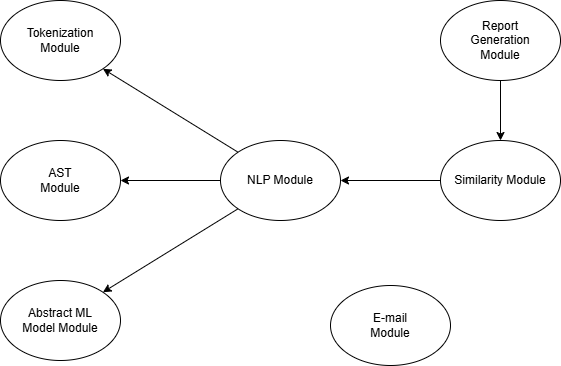
\includegraphics[width=\textwidth]{../Assets/BackEndHierarchy.png}
\caption{Use hierarchy among back end modules}
\label{FigUH}
\end{figure}



\begin{figure}[H]
  \centering
  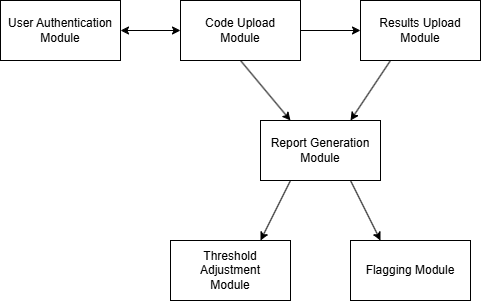
\includegraphics[width=0.5\textwidth]{../Assets/FrontEndHierarchy.png}
  \caption{Use hierarchy among front end modules}
  \label{FigUH}
  \end{figure}

%\section*{References}
\newpage
\section{User Interfaces}
The below are mockups of the user interface for the software and are subject to change based on user feedback and design decisions.

\begin{figure}[H]
  \centering
  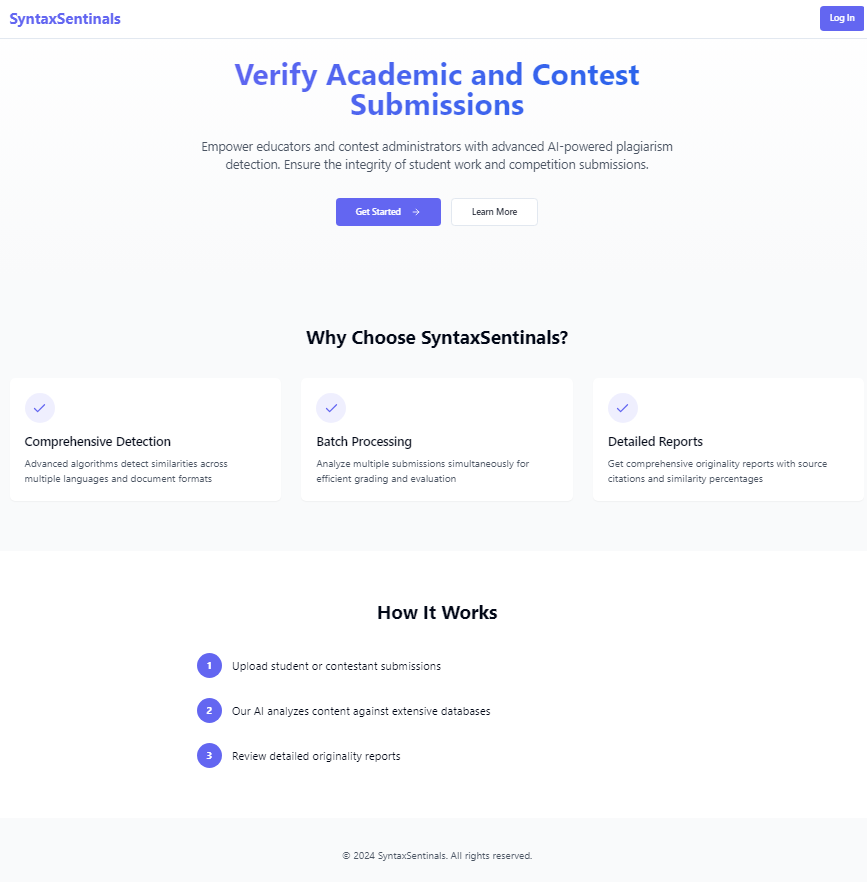
\includegraphics[width=\textwidth]{Landing.png}
  \caption{Landing Page}
  \label{fig:landing}
\end{figure}

\begin{figure}[H]
  \centering
  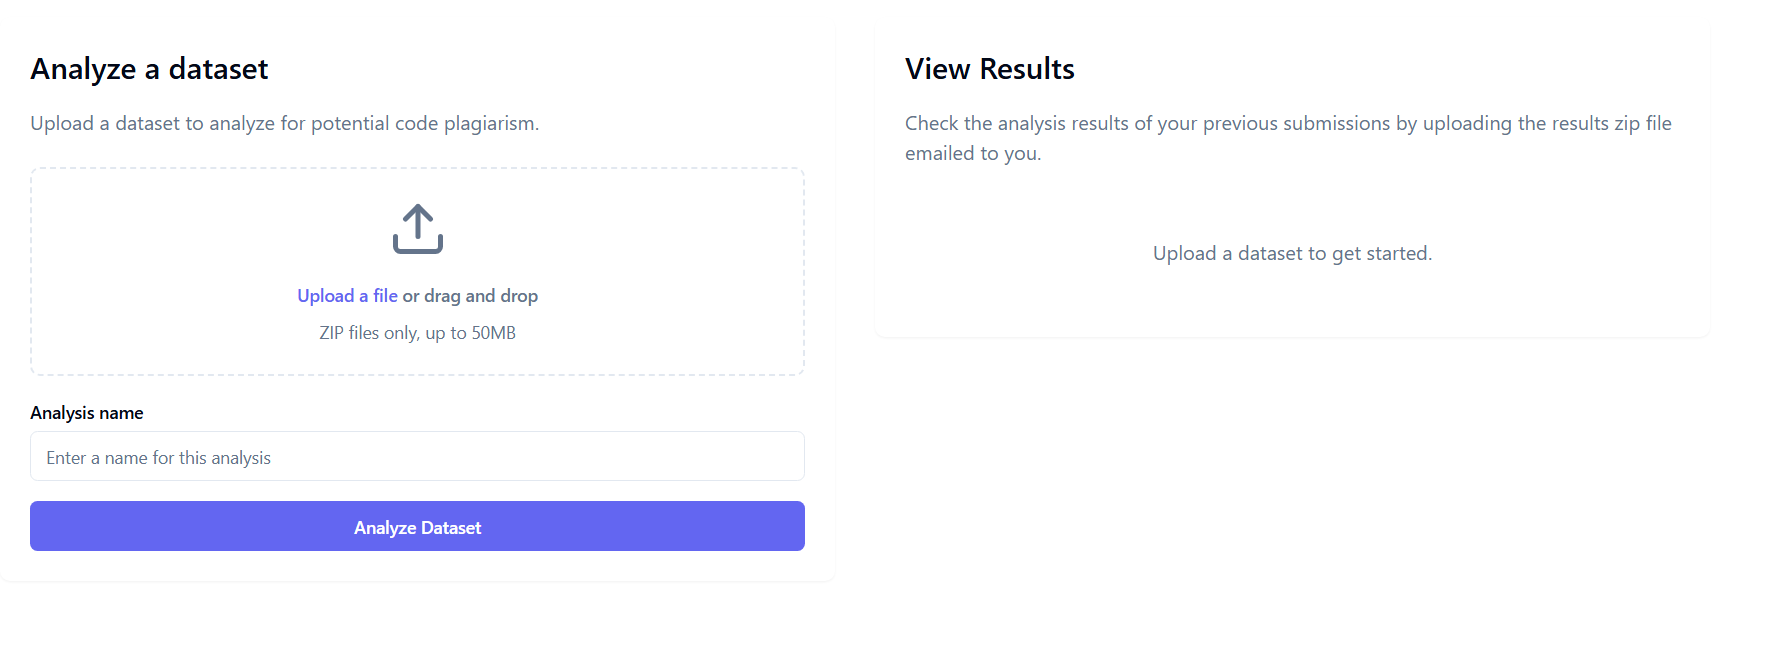
\includegraphics[width=\textwidth]{home.png}
  \caption{Home Page}
  \label{fig:home}
\end{figure}

\begin{figure}[H]
  \centering
  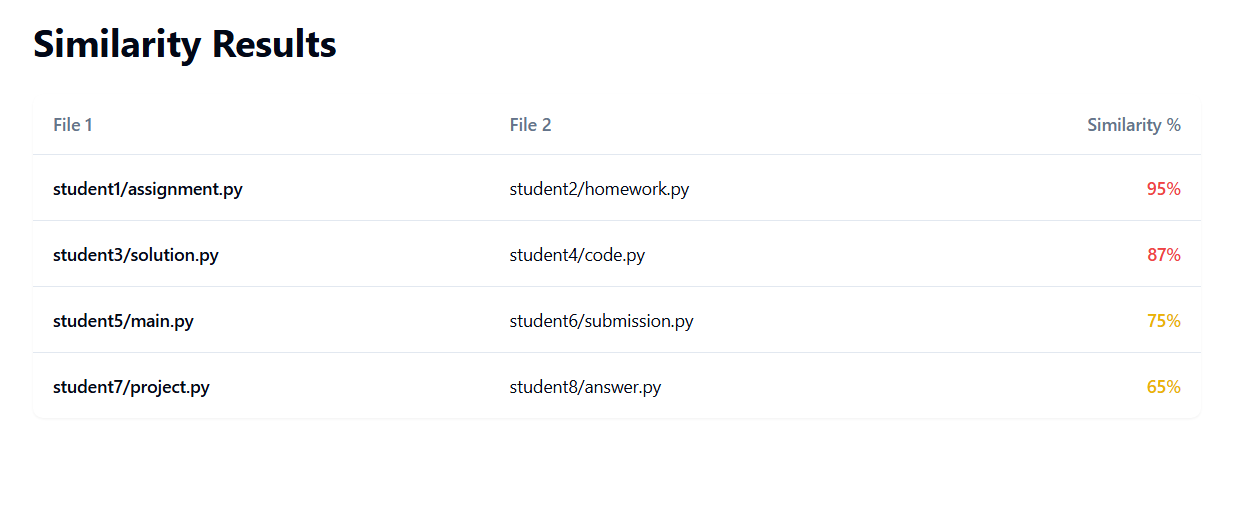
\includegraphics[width=\textwidth]{results.png}
  \caption{Results Page}
  \label{fig:results}
\end{figure}

\begin{figure}[H]
  \centering
  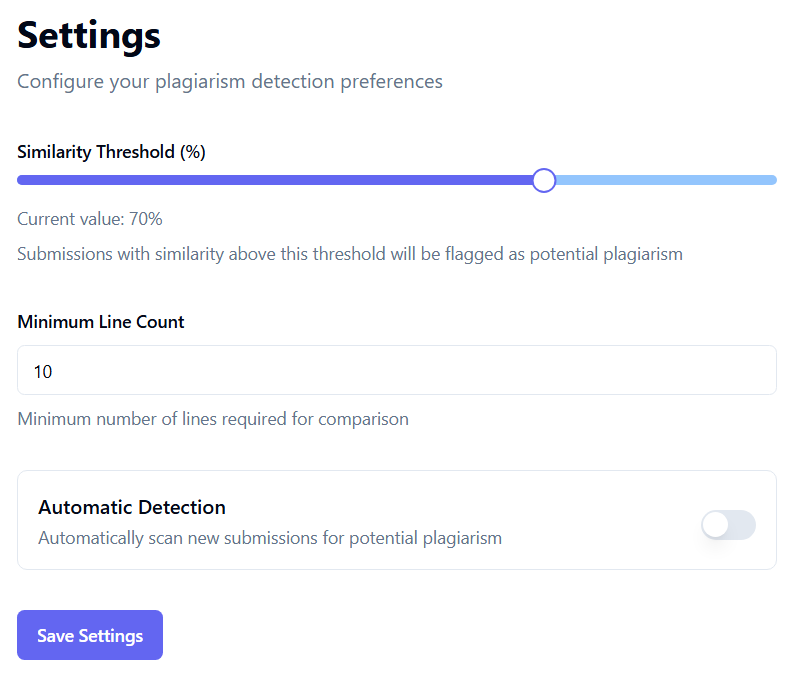
\includegraphics[width=\textwidth]{settings.png}
  \caption{settings Page}
  \label{fig:results}
\end{figure}

\section{Design of Communication Protocols}

This section outlines the external services that will be used by the software and their respective purposes.

\subsection{External Services Overview}
The system will integrate with Auth0 to enhance functionality and provide a seamless user experience.

\subsection{Authentication Service: Auth0}
Auth0 will be used for user authentication and authorization. It provides secure login, single sign-on (SSO), and multi-factor authentication (MFA) capabilities. Auth0 will handle user credentials and ensure that only authorized users can access the system.

\subsection{Integration and Security}
Auth0 will be integrated using its Javascript SDK. Secure communication channels (e.g., HTTPS) will be used to protect data in transit. Additionally, proper authentication and authorization mechanisms will be implemented to ensure that only authorized components can interact with Auth0.

\section{Timeline}

% \wss{Schedule of tasks and who is responsible}

\subsection{Module Implementation Timeline (Starting Jan 17)}

\subsubsection{User Interface (UI) Modules}
\begin{itemize}
    \item \textbf{Jan 17 - Jan 20: User Authentication Module (\ref{mAuth})}
    \begin{itemize}
        \item Develop UI for user registration and login.
        \item Integrate with backend authentication services.
        \item \textbf{Responsibility:} Lucas.
    \end{itemize}
    
    \item \textbf{Jan 21 - Jan 25: Code Upload Module (\ref{mCodeUpload})}
    \begin{itemize}
        \item Implement the file upload interface.
        \item Validate and display upload status to the user.
        \item \textbf{Responsibility:} Mohsin.
    \end{itemize}
    
    \item \textbf{Jan 26 - Jan 30: Results Upload Module (\ref{mResultsUpload})}
    \begin{itemize}
        \item Create UI for uploading processed result files.
        \item Display confirmation and errors for invalid uploads.
        \item To finalize this module it requires the completion of \ref{mEmail}
        \item \textbf{Responsibility:} Lucas.
    \end{itemize}
    
    \item \textbf{Jan 31 - Feb 4: Threshold Adjustment Module (\ref{mThreshold})}
    \begin{itemize}
        \item Develop an interface for adjusting similarity thresholds.
        \item Provide sliders or input boxes for customization.
        \item \textbf{Responsibility:} Mohsin.
    \end{itemize}
    
    \item \textbf{Feb 5 - Feb 8: Flagging Module (\ref{mFlagging})}
    \begin{itemize}
        \item Add functionality for users to flag suspicious results.
        \item Ensure flagged items are visually distinct in the UI.
        \item \textbf{Responsibility:} Mohsin.
    \end{itemize}
    
    \item \textbf{Feb 9 - Feb 14: Report Results Module (\ref{mResults})}
    \begin{itemize}
        \item Implement a results display interface with options for sorting and filtering.
        \item Add the ability to download or email reports directly from the UI.
        \item \textbf{Responsibility:} Lucas and Mohsin.
    \end{itemize}
\end{itemize}

\subsubsection{Backend Modules}
\begin{itemize}
    \item \textbf{Jan 17 - Jan 23: NLP Model Module (\ref{mNLP})}
    \begin{itemize}
        \item Finalize and integrate the trained plagiarism detection model.
        \item \textbf{Responsibility:} Dennis, Luigi, and Julian.
    \end{itemize}

    \item \textbf{Jan 17 - Jan 29: Similarity Scoring Module (\ref{mScoring})}
    \begin{itemize}
        \item Process NLP model outputs for similarity scores.
        \item Optimize backend logic for performance.
        \item \textbf{Responsibility:} Dennis, Luigi, and Julian.
    \end{itemize}

    \item \textbf{Jan 30 - Feb 4: Report Generation Module (\ref{mReport})}
    \begin{itemize}
        \item Generate reports based on processed similarity data.
        \item Ensure compatibility with frontend requirements.
        \item \textbf{Responsibility:} Entire team.
    \end{itemize}

    \item \textbf{Feb 5 - Feb 8: Email Sending Module (\ref{mEmail})}
    \begin{itemize}
        \item Develop functionality for sending results via email.
        \item Implement error handling for failed deliveries.
        \item \textbf{Responsibility:} Dennis, Luigi, and Julian.
    \end{itemize}
\end{itemize}

\vspace{0.5cm}


% \wss{You can point to GitHub if this information is included there}

\bibliographystyle {plainnat}
\bibliography{../../../refs/References}

\newpage{}

\end{document}